\question{Câu 2}

Thiết kế mạch tổ hợp tìm vị trí bit 1 đầu tiên (tính từ MSB) của chuỗi 24-bit. Cho các standard cell như sau: cổng not, các cổng logic 2 ngõ vào, mux 2-1, mux 4-1.

\answer{a}{Thiết kế mạch chỉ được dùng các standard cell trên.}

Đầu tiên nhóm em sẽ thiết kế từ một bộ tìm kiếm vị trí bit 1 đầu tiên (tính từ MSB) cho một chuỗi 4-bit trước. 

\begin{table}[H]
	\centering
	\begin{tabular}{|c|c|c|c|c|c|c|}
		\hline
		\multicolumn{4}{|c|}{Input} & \multicolumn{2}{c|}{Output} & Zero Flag \\
		\hline
		$X_{3}$ & $X_{2}$ & $X_{1}$ & $X_{0}$ & $Y_{1}$ & $Y_{0}$ & $V$ \\
		\hline
		0 & 0 & 0 & 0 & 0 & 0 & 1 \\
		\hline
		0 & 0 & 0 & 1 & 0 & 0 & 0 \\
		\hline
		0 & 0 & 1 & X & 0 & 1 & 0 \\
		\hline
		0 & 1 & X & X & 1 & 0 & 0 \\
		\hline
		1 & X & X & X & 1 & 1 & 0 \\
		\hline
	\end{tabular}
	\caption{Bảng sự thật của bộ phát hiện bit 1 (Leading one position) cho 4 bit.}
	\label{tab:leading-one-4bit}
\end{table}

Từ bảng \ref{tab:leading-one-4bit}, ta rút gọn và có được mạch như sau:

\begin{figure}[H]
	\centering
	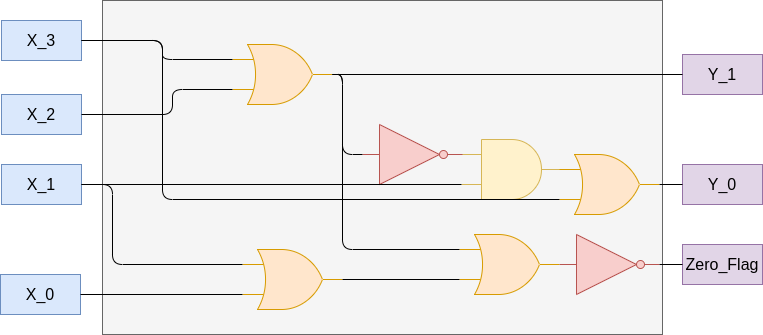
\includegraphics[width=.8\linewidth]{/home/noname/Documents/project_tiny/Ex3/20_doc/my-chapters/my-diagrams/Question2/spec.png}
	\caption{Sơ đồ logic của bộ LOPD 4bit.}
\end{figure}

Từ bộ LOPD 4-bit trên, ta triển khai bộ LOPD 8-bit và bộ LOPD 16-bit như sau:

\begin{figure}[H]
	\centering
	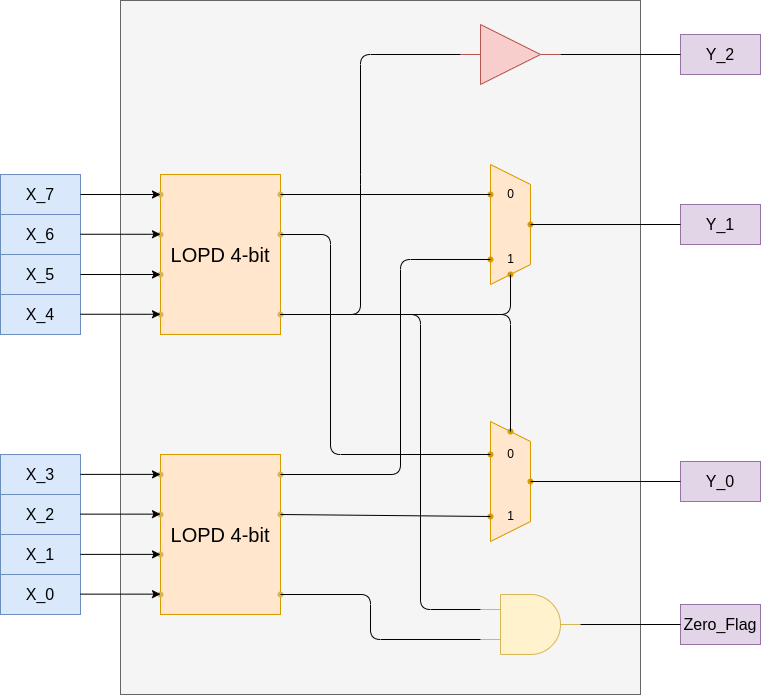
\includegraphics[width=.8\linewidth]{/home/noname/Documents/project_tiny/Ex3/20_doc/my-chapters/my-diagrams/Question2/LOPD_8bit.png}
	\caption{Sơ đồ logic của bộ LOPD 8bit.}
\end{figure}

\begin{figure}[H]
	\centering
	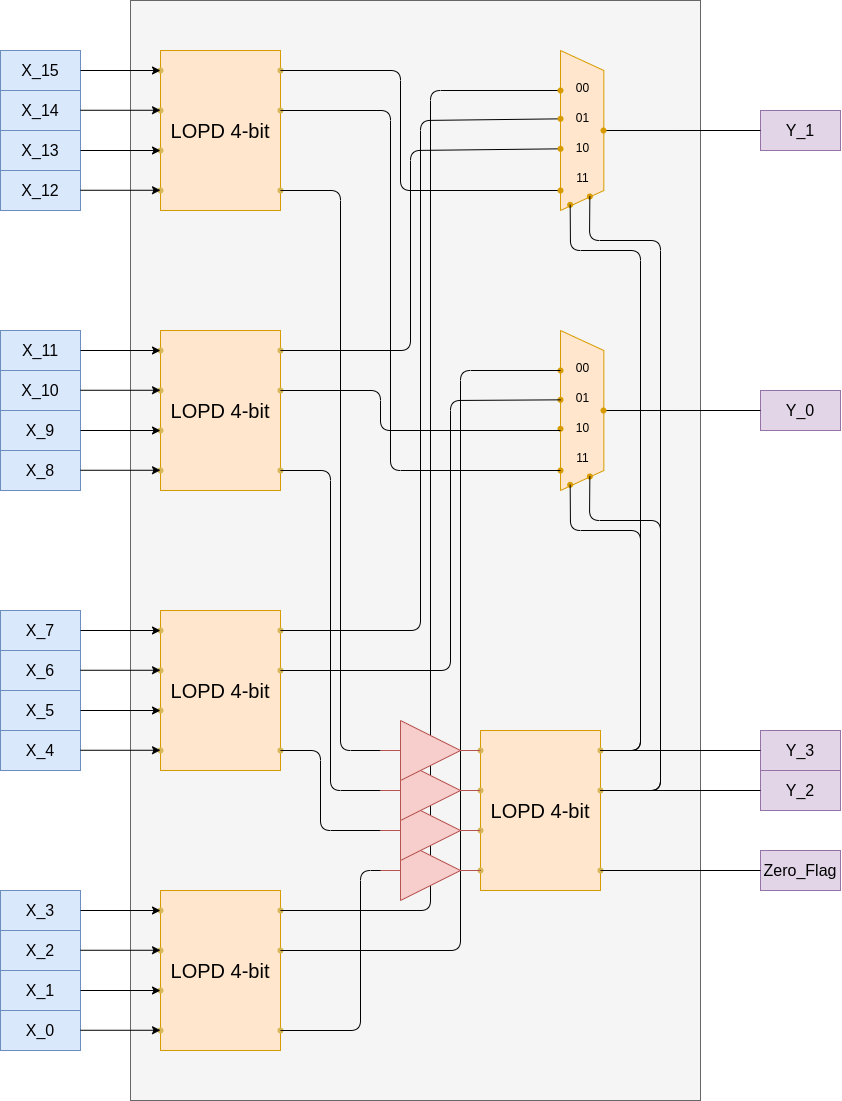
\includegraphics[width=.8\linewidth]{/home/noname/Documents/project_tiny/Ex3/20_doc/my-chapters/my-diagrams/Question2/LOPD_16bit.png}
	\caption{Sơ đồ logic của bộ LOPD 16bit.}
\end{figure}

Từ bộ LOPD 8-bit và LOPD 16-bit trên, ta ghép lại thành 24-bit với LOPD 8-bit vào vị trí 8-bit cao (từ $ 23 \rightarrow 16 $) và bộ LOPD 16-bit vào 16-bit thấp (từ $ 15 \rightarrow 0 $).

\begin{figure}[H]
	\centering
	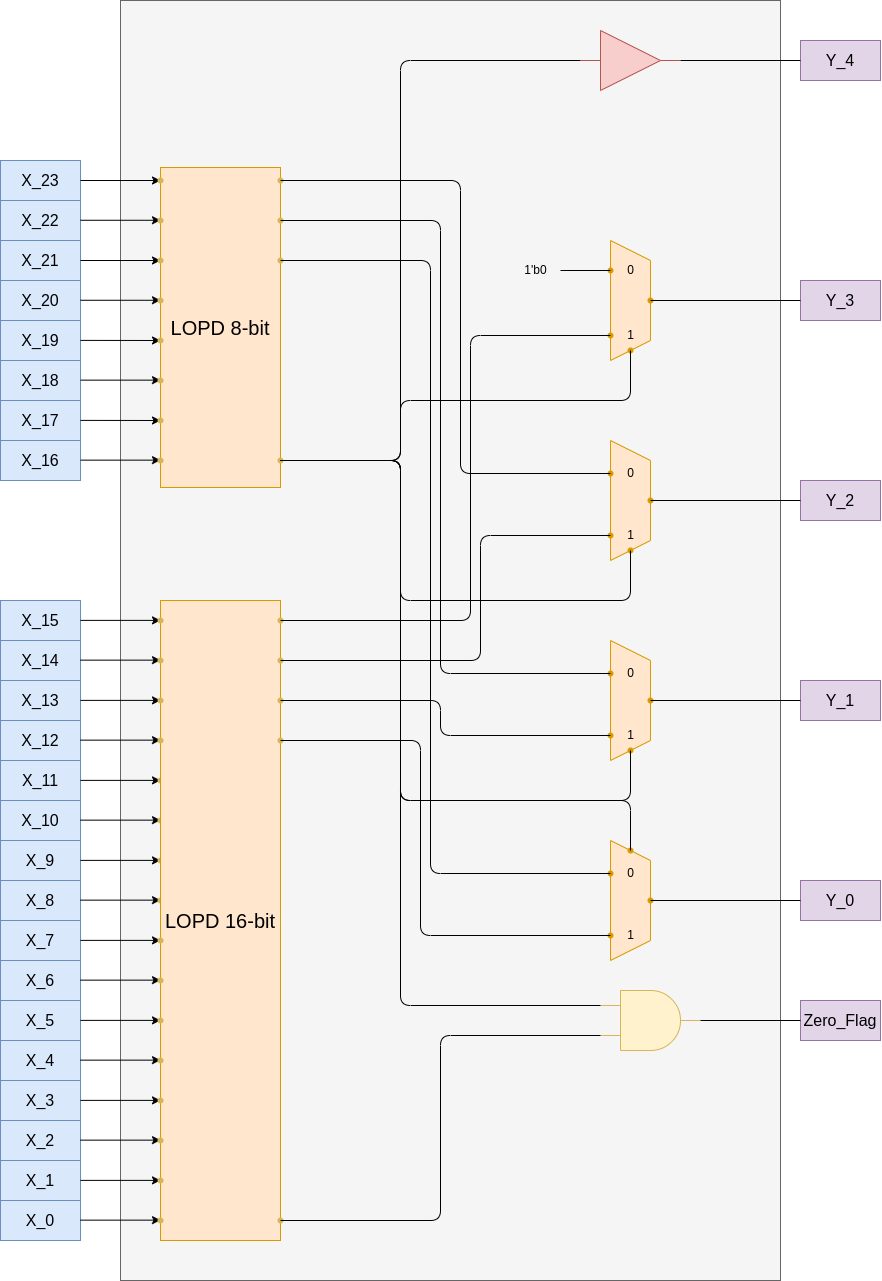
\includegraphics[width=.8\linewidth]{/home/noname/Documents/project_tiny/Ex3/20_doc/my-chapters/my-diagrams/Question2/LOPD_24bit.png}
	\caption{Sơ đồ logic của bộ LOPD 24-bit.}
\end{figure}

\answer{b}{Viết chương trình HDL mô tả mạch đã cho.}

\lstinputlisting[style=StyleCode, language=SystemVerilog, caption={Chương trình mô tả LOPD 4-bit.}]{/home/noname/Documents/project_tiny/Ex3/02_rtl/Question2/LOPD_4bit.sv}

\lstinputlisting[style=StyleCode, language=SystemVerilog, caption={Chương trình mô tả LOPD 8-bit.}]{/home/noname/Documents/project_tiny/Ex3/02_rtl/Question2/LOPD_8bit.sv}

\lstinputlisting[style=StyleCode, language=SystemVerilog, caption={Chương trình mô tả LOPD 16-bit.}]{/home/noname/Documents/project_tiny/Ex3/02_rtl/Question2/LOPD_16bit.sv}

\lstinputlisting[style=StyleCode, language=SystemVerilog, caption={Chương trình mô tả LOPD 24-bit.}]{/home/noname/Documents/project_tiny/Ex3/02_rtl/Question2/Question2.sv}

\answer{c}{Viết testbench cho mạch, thực hiện testbench với 100 mẫu và tính scoreboard của 100 mẫu đó.}

Đầu tiên nhóm em thưc hiện triển khai chứng minh kết quả đúng bằng giải thuật sau:

\begin{lstlisting}[style=StyleCode, language=SystemVerilog, caption={Giải thuật chứng minh kết quả của bộ LOPD 24-bit.}]
	function automatic logic [SIZE_LOP-1:0] Test_LOPD(
		input logic [SIZE_DATA-1:0]     f_i_data
	);
		logic [SIZE_DATA-1:0] t_temp;
		int cnt_position_1;
		begin
			t_temp = f_i_data;
			cnt_position_1 = 0;
			
			if(t_temp == 0) begin
				Test_LOPD = 0;
			end else begin
				while (t_temp[SIZE_DATA-1] == 0) begin
					t_temp = t_temp << 1;
					cnt_position_1 ++;
				end
				Test_LOPD = SIZE_DATA - cnt_position_1 - 1;
			end
		end
	endfunction
\end{lstlisting}

\begin{itemize}[label=-]
	\item TestCase1: Thực hiện test tất cả các giá trị bit 1 với dùng phương pháp shift left để test tất cả các vị trí bit 1 trong 24-bit.
	
	\begin{lstlisting}[style=StyleCode, language=SystemVerilog, caption={Test 24 trường hợp vị trí bit 1 cho bộ LOPD 24-bit.}]
		bit_pos = 1;
		repeat (24) begin
			@(posedge i_clk);
			#1;
			i_addr = i_addr + 1;
			i_data  = bit_pos;
			@(negedge i_clk);
			#1;
			$display("[TIME: %5t] [%s] i_data = %b (%d) \t| o_one_position = %b (%d) \t| o_zero_flag = %b", $time, "Direcly", i_data, i_data, o_one_position, o_one_position, o_zero_flag);
			$display("=> %4s: Expect: %8h, DUT: %8h ", (Test_LOPD(i_data) == o_one_position) ? "PASS" : "FAIL", o_one_position, Test_LOPD(i_data));
			test_count = test_count + 1;
			test_pass  = (Test_LOPD(i_data) == o_one_position) ? test_pass + 1 : test_pass;
			bit_pos = bit_pos << 1'b1;
		end
	\end{lstlisting}
	
	Kết quả
	
	\begin{lstlisting}[style=StyleResult, language=SystemVerilog, caption={Kết quả của TestCase1.}]
		[TIME: 41000] [Direcly] i_data = 000000000000000000000001 (       1) 	| o_one_position = 00000 ( 0) 	| o_zero_flag = 0
		=> PASS: Expect: 00000000, DUT: 00000000 
		[TIME: 51000] [Direcly] i_data = 000000000000000000000010 (       2) 	| o_one_position = 00001 ( 1) 	| o_zero_flag = 0
		=> PASS: Expect: 00000001, DUT: 00000001 
		[TIME: 61000] [Direcly] i_data = 000000000000000000000100 (       4) 	| o_one_position = 00010 ( 2) 	| o_zero_flag = 0
		=> PASS: Expect: 00000002, DUT: 00000002 
		[TIME: 71000] [Direcly] i_data = 000000000000000000001000 (       8) 	| o_one_position = 00011 ( 3) 	| o_zero_flag = 0
		=> PASS: Expect: 00000003, DUT: 00000003 
		...
		[TIME: 261000] [Direcly] i_data = 010000000000000000000000 ( 4194304) 	| o_one_position = 10110 (22) 	| o_zero_flag = 0
		=> PASS: Expect: 00000016, DUT: 00000016 
		[TIME: 271000] [Direcly] i_data = 100000000000000000000000 ( 8388608) 	| o_one_position = 10111 (23) 	| o_zero_flag = 0
		=> PASS: Expect: 00000017, DUT: 00000017 
	\end{lstlisting}

	\item TestCase2: Thực hiện test ngẫu nhiên giá trị đầu vào.
	
	\begin{lstlisting}[style=StyleCode, language=SystemVerilog, caption={Test 100 trường hợp đầu vào ngẫunhiên cho bộ LOPD 24-bit.}]
		repeat (100) begin
			@(posedge i_clk);
			#1;
			bit_pos = $urandom_range(0, SIZE_DATA-1);
			i_data = 24'b1 << bit_pos;
			if ($urandom_range(0, 1)) begin
			i_data |= $urandom_range(0, (1 << SIZE_DATA) - 1);
			end
			#5;
			$display("[TIME: %5t] [%s] i_data = %b (%d) \t| o_one_position = %b (%d) \t| o_zero_flag = %b", $time, "Random", i_data, i_data, o_one_position, o_one_position, o_zero_flag);
			$display("=> %4s: Expect: %8h, DUT: %8h ", (Test_LOPD(i_data) == o_one_position) ? "PASS" : "FAIL", o_one_position, Test_LOPD(i_data));
			test_count = test_count + 1;
			test_pass  = (Test_LOPD(i_data) == o_one_position) ? test_pass + 1 : test_pass;
			i_addr = i_addr + 1;
		end
	\end{lstlisting}

	Kết quả
	
	\begin{lstlisting}[style=StyleResult, language=SystemVerilog, caption={Kết quả của TestCase2.}]
		[TIME: 281000] [Random] i_data = 000100000000000000000000 ( 1048576) 	| o_one_position = 10100 (20) 	| o_zero_flag = 0
		=> PASS: Expect: 00000014, DUT: 00000014 
		[TIME: 291000] [Random] i_data = 000000000000000000000100 (       4) 	| o_one_position = 00010 ( 2) 	| o_zero_flag = 0
		=> PASS: Expect: 00000002, DUT: 00000002 
		[TIME: 301000] [Random] i_data = 000000000000000000000001 (       1) 	| o_one_position = 00000 ( 0) 	| o_zero_flag = 0
		=> PASS: Expect: 00000000, DUT: 00000000 
		[TIME: 311000] [Random] i_data = 010000000000000000000000 ( 4194304) 	| o_one_position = 10110 (22) 	| o_zero_flag = 0
		=> PASS: Expect: 00000016, DUT: 00000016  
		...
		[TIME: 1241000] [Random] i_data = 010000000000000000000000 ( 4194304) 	| o_one_position = 10110 (22) 	| o_zero_flag = 0
		=> PASS: Expect: 00000016, DUT: 00000016 
		[TIME: 1251000] [Random] i_data = 000000000100000000000000 (   16384) 	| o_one_position = 01110 (14) 	| o_zero_flag = 0
		=> PASS: Expect: 0000000e, DUT: 0000000e 
		[TIME: 1261000] [Random] i_data = 000000100000000000000000 (  131072) 	| o_one_position = 10001 (17) 	| o_zero_flag = 0
		=> PASS: Expect: 00000011, DUT: 00000011 
		[TIME: 1271000] [Random] i_data = 000000000010000000000000 (    8192) 	| o_one_position = 01101 (13) 	| o_zero_flag = 0
		=> PASS: Expect: 0000000d, DUT: 0000000d 
	\end{lstlisting}

	\item Kết quả tổng kết.
	
	\begin{lstlisting}[style=StyleResult, language=SystemVerilog, caption={Kết quả của tổng kết của bài test.}]
		================================
		==========TEST SUMMARY==========
		Total test cases:    124    
		Passed          :    124    
		Failed          :      0    
		Pass rate       : 100.00%
		================================
	\end{lstlisting}
\end{itemize}